\documentclass[a4paper]{article}
    \usepackage{geometry}
    \usepackage{fancyhdr}
    \usepackage{amsmath,amsthm,amssymb}
    \usepackage{graphicx}
    \usepackage{float}
    \usepackage{subcaption}
    \usepackage{hyperref}
    \usepackage{xcolor}
    \usepackage{titlesec}
    \titleformat{\section}[block]{\color{blue}\Large\bfseries\filcenter}{}{1em}{}
    \titleformat{\subsection}[hang]{\bfseries}{}{1em}{}
    \setcounter{secnumdepth}{0}
    
    \title{Capstone Project\\
        \small Machine Learning Engineer Nanodegree}
    \author{Vitaly Kovalev}
    \date {\today}
    
    \begin{document}
    \maketitle
    % \newpage
    
    \section{Definition}
    \subsection*{Project Overview}
    
    Mass spectrometry is an analytical technique that ionizes chemical or biological material and
    measures mass-to-charge ratio (m/z) of ions (mass spectrum). In simple terms, a mass spectrum
    measures distribution of masses in a sample. Knowing mass to molecule
    \footnote{Throughout the report we will be using the term \textit{ion} instead of \textit{molecule}
    because it describes the data used in the project more precisely.}
    correspondence makes it possible to use mass spectrometry to annotate all peaks in a spectrum with
    molecules they can originate from.
    
    \href{https://ms-imaging.org/wp/}{Mass spectrometry imaging (MSI)} is a technique used 
    in mass spectrometry to visualize
    spatial distribution of masses (or molecules) in a sample. In MSI, a dataset can be represented as
    a 3-dimensional tensor ($N \times M \times K$). Where $N$ and $M$ are spatial dimensions
    (acquisition matrix) and K is a mass dimension ($m/z$ bins). What is unusual about these images
    is that number of channels always exceeds spatial size of images. At the same time, the number
    of mass channels most of the time is excessive and can be reduced.
    
    Pretty often during MSI acquisition, spectra are collected from a sample and its nearby area.
    Also some instruments are restricted to rectangular acquisition areas only.
    This leads to a problem of separation of signals (spectra) coming from the sample itself
    from background signals coming primarily from the nearby area.
    
    European project \href{http://metaspace2020.eu}{METASPACE} aims to provide information about
    spatial distribution of small molecules of biological origin (metabolites) in
    samples provided by users in the form of MSI datasets. Implementation of a method for
    distinguishing between molecules coming from sample and background molecules could greatly
    improve quality of MSI data annotation provided by METASPACE.
    
    \subsection*{Problem Statement}
    
    \begin{figure}[H]
        \centering
        \caption{A “slice” of an MSI dataset for a specific $m/z$ (or associated ion).
        The inner part of manually outlined region (in red) is a sample area, the outside area
        is off sample (or background).
        Here we have an example of a signal that mostly comes (more intense signals are yellow) from
        the off sample area and thus not particularly interesting to the user.}
        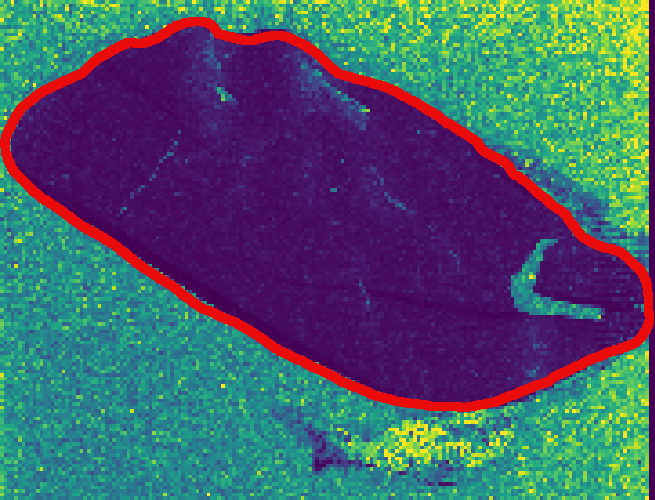
\includegraphics[width=\textwidth,height=4cm,keepaspectratio]{ion_image_1.png}
    \end{figure}
    
    The METASPACE project currently hosts results for more than 3000 MSI datasets. The results
    are represented as a set of images corresponding to different ions. For a number of MSI
    datasets, it is possible to define off sample areas (or images with signal coming from off sample areas)
    using expert knowledge. This way, it is possible to get the ground truth data for the problem in focus.
    
    Originally, each MSI dataset is represented by a 3 dimensional tensor $N \times M \times K$
    with mass measurements for each pixel.
    There are methods to get a binary mask of $N \times M$ shape for the off sample area
    (each pixel assigned one of two classes).
    It is also possible to represent each pixel data as an N dimensional vector.
    In this form, the data can be used to train a binary classification model
    to predict pixel classes (or off sample masks) for new MSI datasets. The available options are
    Logistic Regression, Bayesian Classifier or one of the ensemble classifiers like Random Forest.
    
    It is important to mention that the data in its original form does not contain pixel labels
    (MSI dataset off sample masks). That is why it is a part of the project to label the data so that
    a supervised algorithm can be used.
    
    \pagebreak
    \subsection*{Metrics}
    
    Model performance can be measured the same way as in any other binary classification task,
    using accuracy, AUC, F1 or precision and recall scores.
    
    \begin{figure}[H]
        \centering
        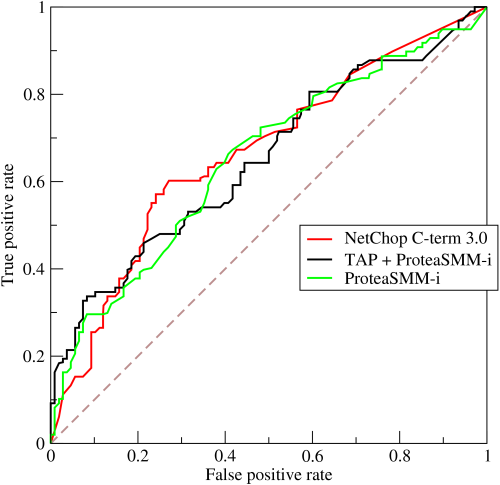
\includegraphics[width=\textwidth,height=5cm,keepaspectratio]{roccurves.png}
        \caption{An example of three ROC curves for a binary classification problem.
        Area Under the Curve (AUC) - the area under each line. The higher the value
        of AUC the better the model.}
    \end{figure}
    
    \begin{equation*}
    Precision = \frac{TP}{TP + FP},\ TP - true\ positives,\ FP - false\ positives
    \end{equation*}
    
    \begin{equation*}
    Recall = \frac{TP}{TP + FN},\ TP - true\ positives,\ FN - false\ negatives
    \end{equation*}
    
    \begin{equation*}
    F_1 = 2 \cdot \frac{precision \cdot recall}{precision + recall}
    \end{equation*}
    
    It is also a part of the project to define the most adequate and accurate metric.
    AUC is a pretty common metric to use but like accuracy it might be affected by imbalanced class distribution.
    F1 is more robust metric in this sense. A pair of two metrics, recall and precision, can be
    used in cases when the requirements to the problem solution are defined like this 
    "find a model with highest precision given that recall is not lower than 0.8".
    The last formulation suits the project problem.
    
    \pagebreak
    \section*{Analysis}
    
    \subsection*{Data Exploration}
    
    To solve the problem defined above, a subset of 50 MSI datasets was collected, one dataset per
    MSI experiment. So the target dataset contains data from multiple MSI datasets.
    Each MSI dataset contains several
    thousand measurements or mass spectra acquired on a regular two-dimensional grid. One spectrum is
    a one-dimensional vector with thousands elements. Each spectrum (or pixel) is located on the sample
    or off sample (background) area. So each pixel can be assigned one of the two classes (on/off sample).
    
    \begin{figure}[H]
        \centering
            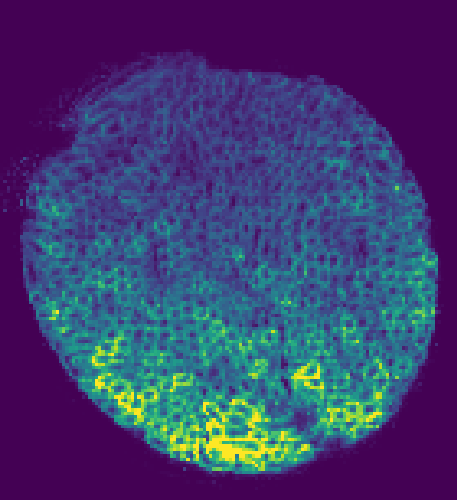
\includegraphics[width=\textwidth,height=4cm,keepaspectratio]{ion_image_2.png}
        \caption{$m/z$ (ion) image example}
    \end{figure}
    
    \begin{figure}[H]
        \centering
            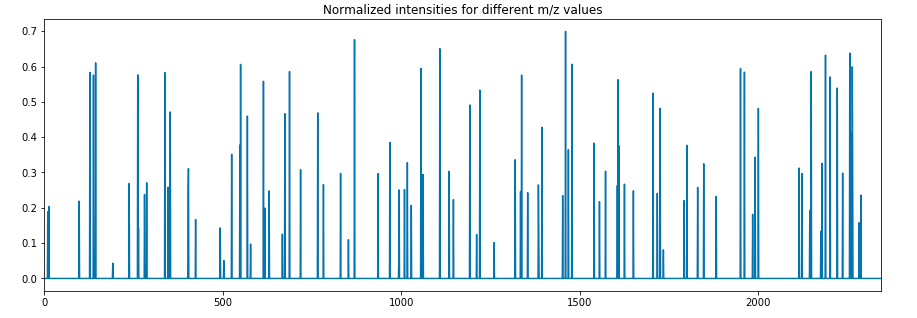
\includegraphics[width=1.\textwidth]{spectrum_graph_1.png}
        \caption{Single (normalized) spectrum example}
    \end{figure}
    
    The MSI datasets can be aquired with different instruments in quite different conditions, biological
    samples can also be very diverse. Because of this, spectra (pixels) that have the same class but belong
    to different MSI datasets can be pretty unsimilar. Additional difficulties are caused by some MSI datasets
    being not rectangular but of arbitrary shape. Which makes off sample areas around sample in those datasets
    really small. The amount of signal for every MSI dataset can be quite different as well. This makes 
    comparison of spectra between MSI datasets a challenging task.
    
    \subsection*{Exploratory Visualization}
    
    \begin{figure}[H]
        \caption{Two images above are slices of MSI datasets of regular and irregular shapes.
        It is pretty easy to see
        two distinct areas on the first image. On the second one, it is tough to locate the off sample area as
        it is represented only with a thin ring around the sample.}
        \begin{subfigure}[b]{0.5\textwidth}
            \centering
            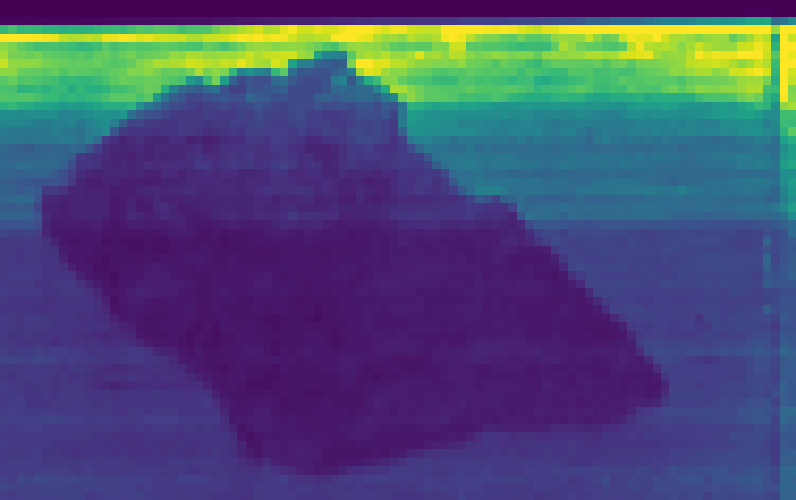
\includegraphics[width=\textwidth,height=4cm,keepaspectratio]{ion_image_regular.png}
            \caption{Rectangular MSI dataset}
            \label{fig:ion_image_regular.png}
        \end{subfigure}
        \begin{subfigure}[b]{0.5\textwidth}
            \centering
            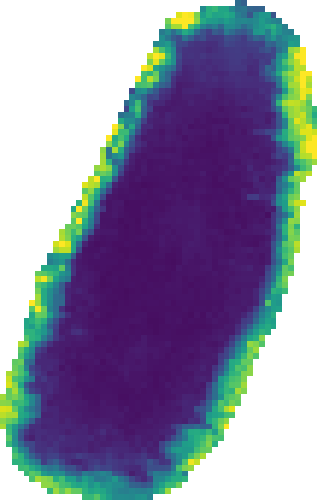
\includegraphics[width=\textwidth,height=4cm,keepaspectratio]{ion_image_irregular.png}
            \caption{Irregular shape MSI dataset}
            \label{fig:ion_image_irregular.png}
        \end{subfigure}
    \end{figure}
    
    \begin{figure}[H]
        \begin{subfigure}[b]{\textwidth}
            \centering
            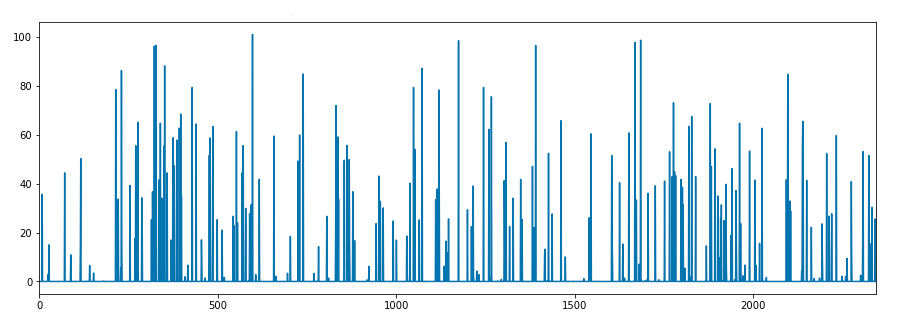
\includegraphics[width=\textwidth,height=5cm,keepaspectratio]{sum_ints_on_sample_graph.png}
            \caption{Sum of on sample spectra}
            \label{fig:sum_ints_on_sample_graph.png}
        \end{subfigure}
        \begin{subfigure}[b]{\textwidth}
            \centering
            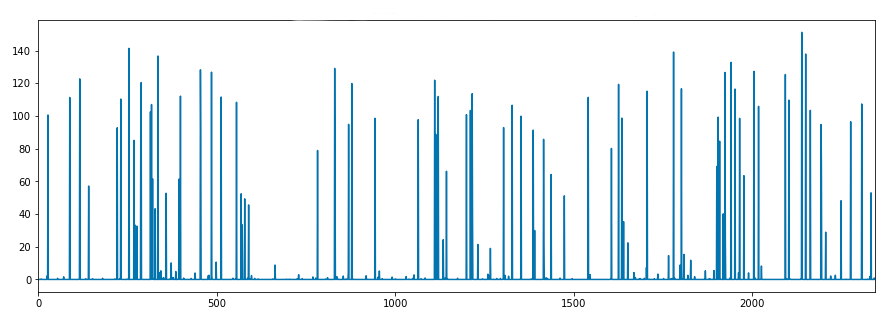
\includegraphics[width=\textwidth,height=5cm,keepaspectratio]{sum_ints_off_sample_graph.png}
            \caption{Sum of off sample spectra}
            \label{fig:sum_ints_off_sample_graph.png}
        \end{subfigure}
        \caption{The above two images show sum of spectra for two areas (on/off sample) of a MSI dataset.
        It is easy to see that there is a difference between these two spectra.}
    \end{figure}
    
    \begin{figure}[H]
        \centering
            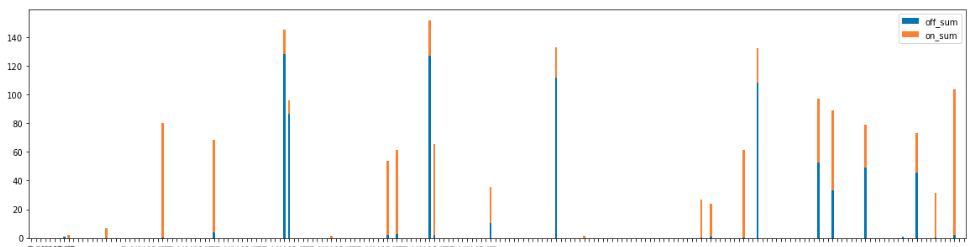
\includegraphics[width=\textwidth,height=5cm]{sum_int_stacked_bar.png}
        \caption{The stacked bars graph is a zoomed version of the above two spectra combined.
        On this graph, it is easier to see that some signals (at specific $m/z$) come mostly from
        the off sample while others from the on sample area.}
    \end{figure}
    
    \begin{figure}[H]
        \centering
            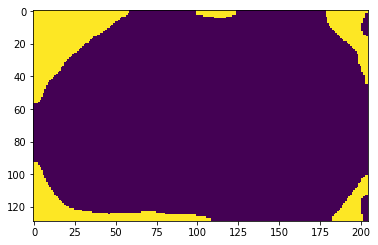
\includegraphics[height=4cm]{off_sample_mask_1.png}
        \caption{The example mask for a MSI dataset, the mask is in yellow.
        Each pixel has one of the two classes assigned to it.
        Correct prediction of such masks for all MSI datasets in focus is one way
        of solving the original problem. Once we have a mask image for a MSI dataset,
        it should be possible to combine it with every result image (ion image)
        from METASPACE for the dataset and decide
        if the image depicts the off sample or the on sample area.}
    \end{figure}
    
    \begin{figure}[H]
        \begin{subfigure}[b]{0.5\textwidth}
            \centering
            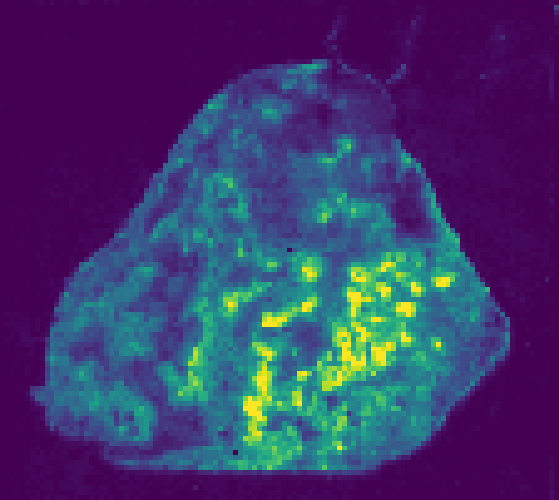
\includegraphics[width=\textwidth,height=4cm,keepaspectratio]{ion_image_on_sample.png}
            \caption{Ion image of the on sample area}
        \end{subfigure}
        \begin{subfigure}[b]{0.5\textwidth}
            \centering
            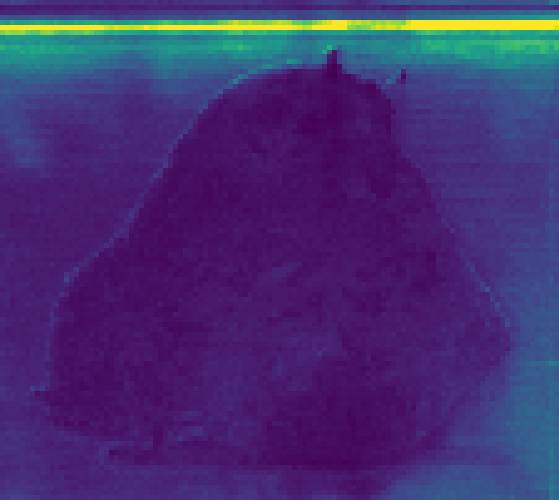
\includegraphics[width=\textwidth,height=4cm,keepaspectratio]{ion_image_off_sample.png}
            \caption{Ion image of the off sample area}
        \end{subfigure}
        \caption{Another approach would be to try to train a model that takes an ion image as input
        and classifies it as on/off sample one.
        Two images from the same MSI dataset, the left one depicts the on sample area,
        the right off sample.}
    \end{figure}
    
    \begin{figure}[H]
        \centering
            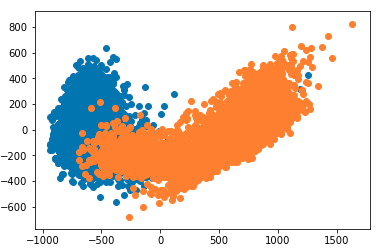
\includegraphics[width=\textwidth,height=6cm,keepaspectratio]{pca_2d_plot.png}
        \caption{The PCA tranformation was applied to all pixels of a MSI dataset.
        Visualisation of the first two components.
        Pixels that belong to different classes have different colour. Here we can clearly see two groups that also have a substantial overlapping.}
    \end{figure}
    
    \begin{figure}[H]
        \centering
            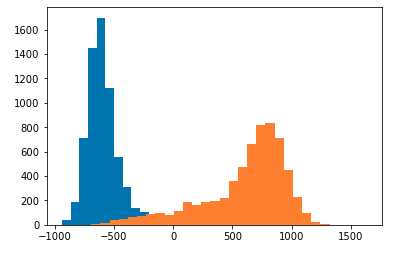
\includegraphics[width=\textwidth,height=6cm,keepaspectratio]{pca_1d_plot.png}
        \caption{A histogram of the first principal component. It is easy to see that distributions of of component values are
        quite different for the classes. Unfortunately, not for all MSI datasets in focus it is possible to get such
        a nice binomial distribution. Another problem with this approach is in the fact that it is not known which 
        class a particular distribution represents, on or off sample. The order of distribution peaks is different for
        each MSI dataset.}
    \end{figure}
    
    \begin{figure}[H]
        \centering
            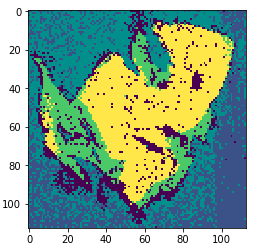
\includegraphics[width=\textwidth,height=6cm,keepaspectratio]{kmeans_cluster_image.png}
        \caption{Another attempt to use unsupervised learning in order to separate pixels of two different classes.
        K-means clustering algorithm with $N=5$ ($N$ - number of clusters) was applied to an MSI dataset.
        The cluster numbers were assigned colours and mapped back to the original pixel locations.
        One can clearly see a nice grouping of pixels. Here the clusters assigned yellow, green and
        dark blue colours together represent on sample area.}
    \end{figure}
    
    \subsection*{Algorithms and Techniques}
    
    As mentioned before, the original problem has two versions:
    \begin{itemize}
        \item Prediction of an off sample mask and using this mask to split all ion images
    into two groups (on and off sample).
        \item Taking ion images as input and directly classifying them into two groups.
    \end{itemize}
    
    For the first version of the problem, it is easier to apply a machine learning technique as
    the off sample mask is simply all MSI dataset pixels with one of the two classes assigned to them.
    So the algorithms for independent classification of pixels were explored. The input vectors 
    for pixel examples were intensities of different ions, an improved version of the pixel mass spectrum.
    In this form, any binary classification algorithm can be applied.
    Wide range of models from scikit-learn Python package have been applied.
    The most satisfying results were obtained with Random Forest, Naive Bayes Classifier and Fully
    Connected Neural Network.
    
    The second step of mask application to ion images, that initially seemed easy, appeared to be
    quite challenging and achievement of good results was not possible.
    That is why the second version of the original problem was explored more thoroughly.
    
    Since inputs were two dimensional single channel images, the available options for models were limited.
    At the moment, Convolutional Neural Networks (CNNs) dominate the field of image recognition and classification.
    \footnote{"Review of Deep Learning Algorithms for Image Classification"
        \url{https://medium.com/comet-app/review-of-deep-learning-algorithms-for-image-classification-5fdbca4a05e2}}
    Python package Keras with TensorFlow as a back-end was used as the easiest way to start experimenting with CNNs.
    
    When people talk about deep learning magically solving one more problem with significant improvement
    over previous approaches, most of the time it will be Deep Convolutional Neural Networsk (CNNs).
    General ideas and the images below are taken from the Data Science and Robots blog,
    courtesy of Brandon Rohrer
    \footnote{\url{https://brohrer.github.io/how_convolutional_neural_networks_work.html}}
    
    \begin{figure}[H]
        \centering
            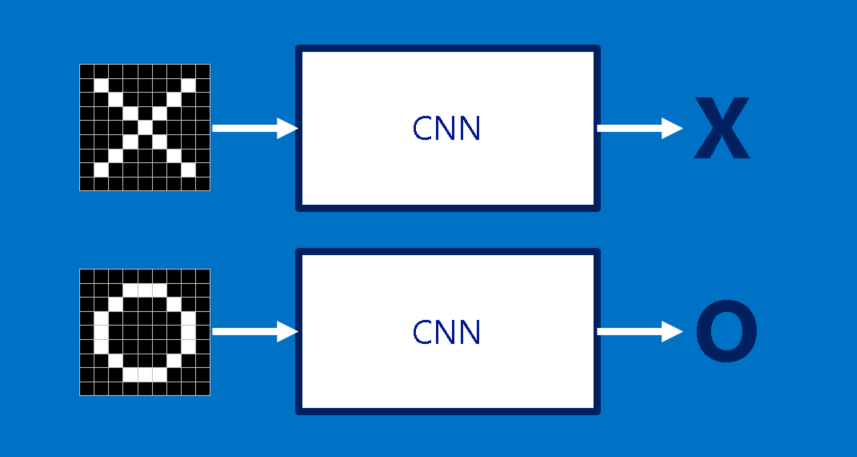
\includegraphics[width=\textwidth,height=2.5cm,keepaspectratio]{cnn1.png}
        \caption{A simple illustration of how CNNs work. Two dimensional array (image) as input,
        a class label as output. Once we have fed enough example images with class labels to the
        networks, it will hopefully learn (adjust all its weights) to predict classes for new
        images it has never seen.}
    \end{figure}
    
    \begin{figure}[H]
        \centering
            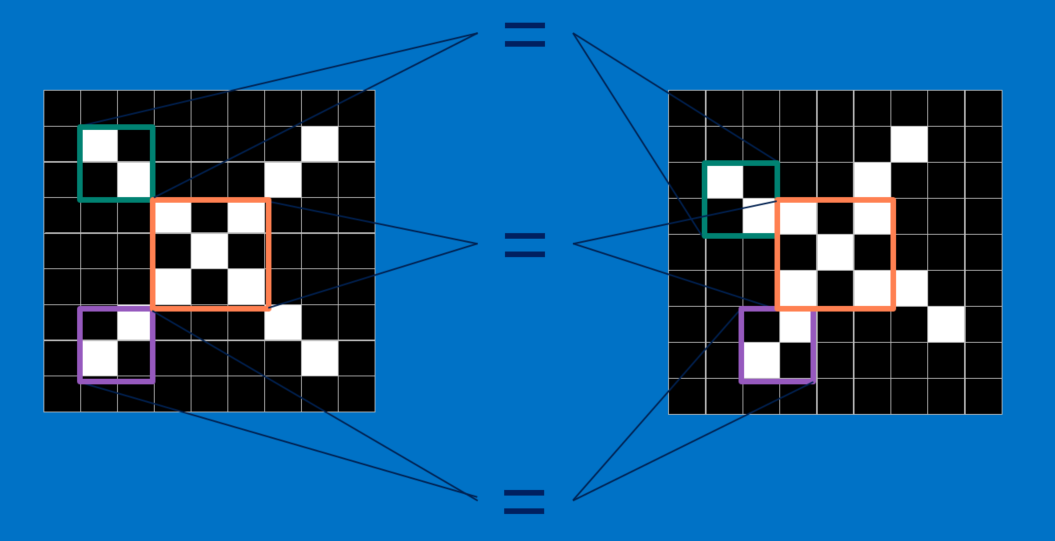
\includegraphics[width=\textwidth,height=2.5cm,keepaspectratio]{cnn3.png}
        \caption{The core concept of CNNs is image features. One can think of them as a set of small images that
        that can be extracted from an input image. They can be located in different places on images but
        still images that have a lot of features in common are considered to be similar. The approach
        of comparing images by features is much more flexible than full image matching schemes.}
    \end{figure}
    
    \begin{figure}[H]
        \centering
            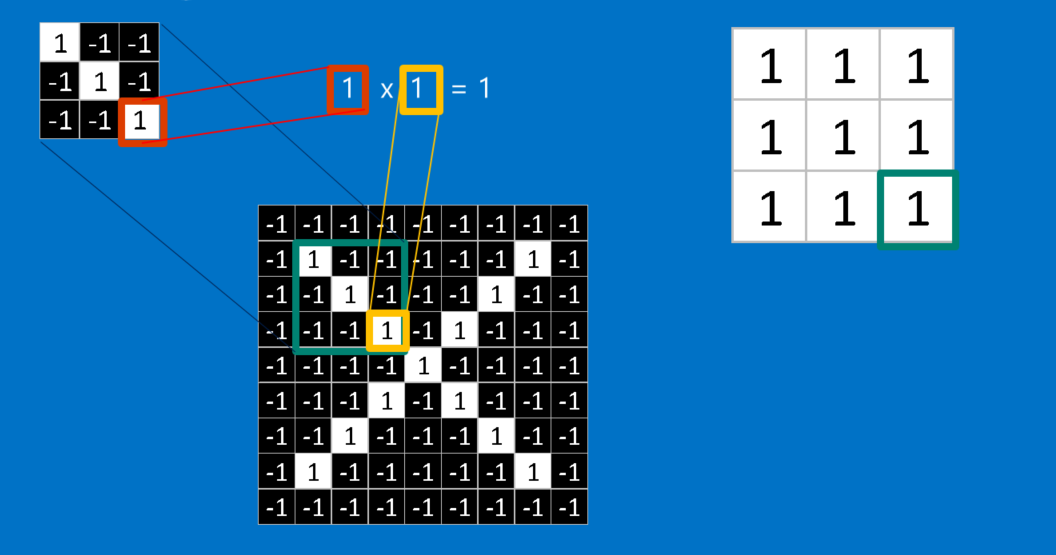
\includegraphics[width=\textwidth,height=2.5cm,keepaspectratio]{cnn5.png}
        \caption{Convolution is another concept that actually gives the name to the CNNs.
        Convolution is a way of detecting particular features on images. For that convolutional filters
        are used, see top left corner. Simple mathematical operations of element-wise multiplication
        and averaging among all results of the filter application are used for that.}
    \end{figure}
    
    \begin{figure}[H]
        \centering
            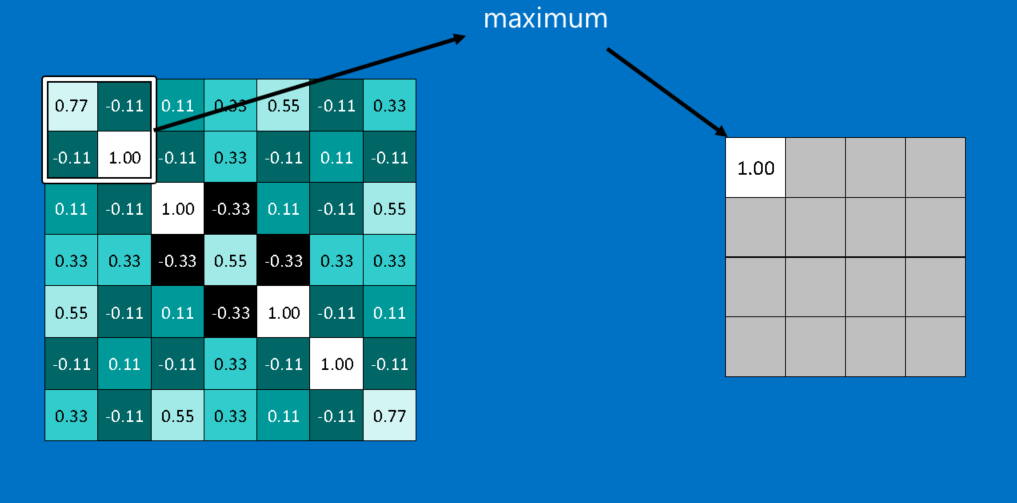
\includegraphics[width=\textwidth,height=2.5cm,keepaspectratio]{cnn8.png}
        \caption{Pooling is a technique used in CNN in order to compensate for feature shifts 
        and distortions.}
    \end{figure}
    
    \begin{figure}[H]
        \centering
            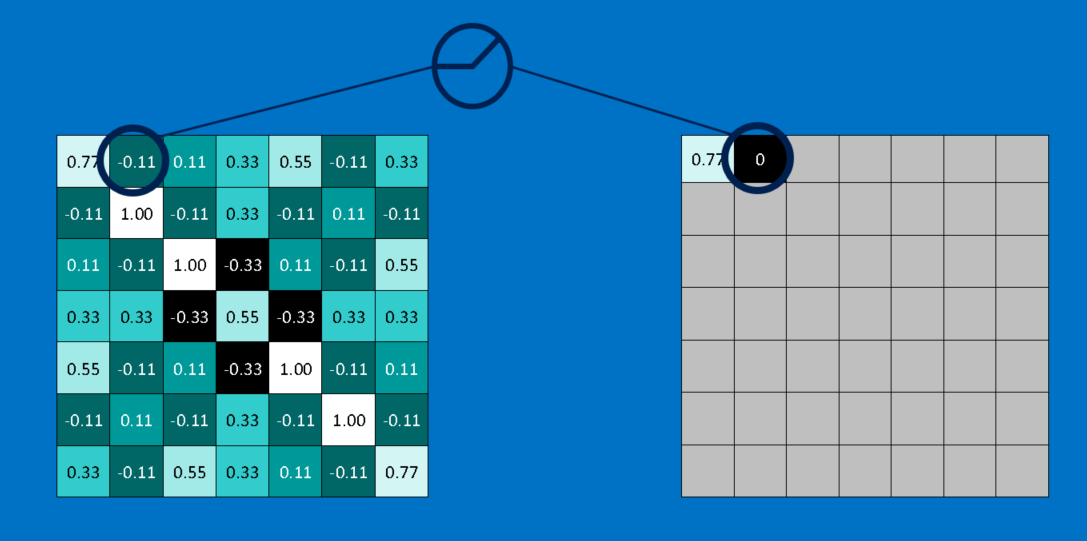
\includegraphics[width=\textwidth,height=2.5cm,keepaspectratio]{cnn10.png}
        \caption{Rectified Linear Units (ReLUs). At every convolutional layer after linear operations
        a non-linear function is applied to the result. ReLUs give CNNs power to capture
        non-linear relations by simply setting any negative number to zero and not changing
        positive numbers.}
    \end{figure}
    
    \begin{figure}[H]
        \centering
            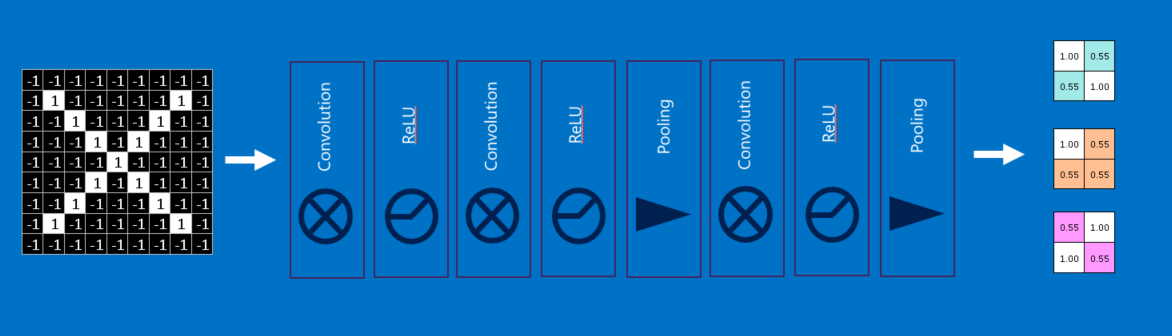
\includegraphics[width=\textwidth,height=2.5cm,keepaspectratio]{cnn12.png}
        \caption{By stacking multiple layers CNNs represent increasingly sophisticated aspects of
        input images. As outputs from previous layers become inputs for the following ones, the network
        learns to detect more and more complex features at each layer.}
    \end{figure}
    
    \begin{figure}[H]
        \centering
            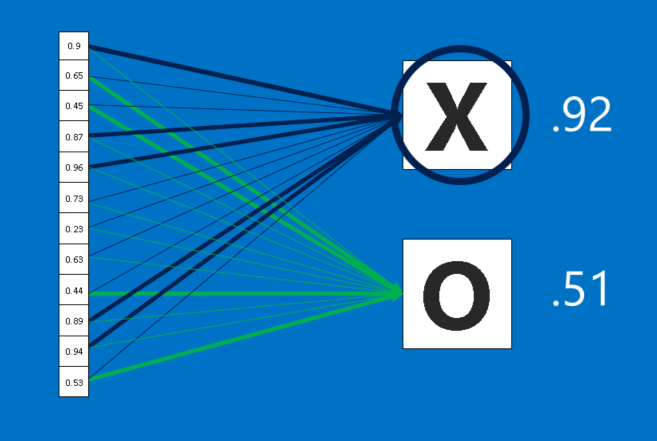
\includegraphics[width=\textwidth,height=2.5cm,keepaspectratio]{cnn13.png}
        \caption{The final layer of any CNN is a dense layer where all the high level features are multiplied
        by weights and the final votes are made in order to decide on image class.}
    \end{figure}
    
    \begin{figure}[H]
        \centering
            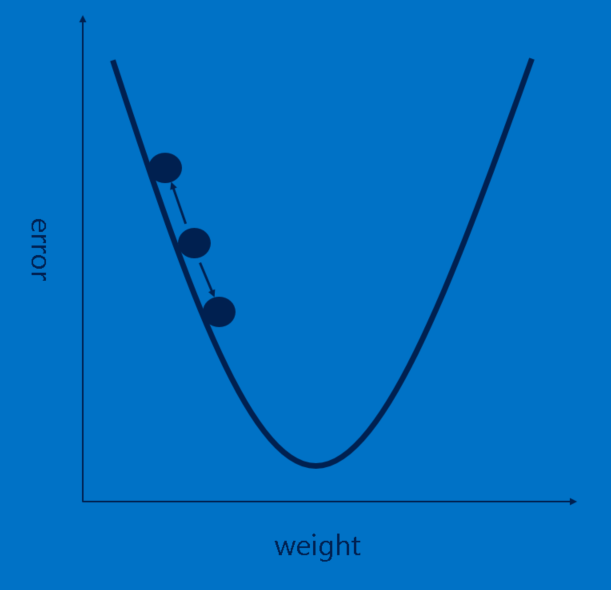
\includegraphics[width=\textwidth,height=2.5cm,keepaspectratio]{cnn15.png}
        \caption{Backpropagation is the algorithm for learning all those parameters the network has.
        It gets its name from the way it propagates errors from the final layer, where we compare predicted
        class labels with actual ones, all the way back to the first layer. The higher the error is at
        a specific layer for a specific image the more parameters of this layer will be corrected.}
    \end{figure}
    
    
    
    \newpage
    \subsection*{Benchmark}
    
    As a simple benchmark model, binary classifiers like Logistic Regression from scikit-learn were
    tested to predict individual classes of all pixels from the test MSI datasets.
    Classes of predicted labels were used to create off sample masks.
    Correlation of off sample masks and ion images from the test MSI datasets
    with thresholding was used to classify ion images into two classes (on or off sample).
    
    The best models, Random Forest and Fully Connected Neural Network, combined with correlation post-processing
    had similar performance and were used as the base benchmark model that achieved the following best results:
    $recall=0.8$, $precision=0.75$
    
    \section*{Methodology}
    
    \subsection*{Data Preprocessing}
    
    About one hundred MSI datasets from METASPACE were selected to be used in the final model training stage.
    Only MSI datasets of regular shape (rectangular) were used. Further, using expert knowledge,
    all ion images for each MSI dataset were separated into two classes, on and off sample.
    
    \begin{figure}[H]
        \begin{subfigure}[b]{\textwidth}
            \centering
            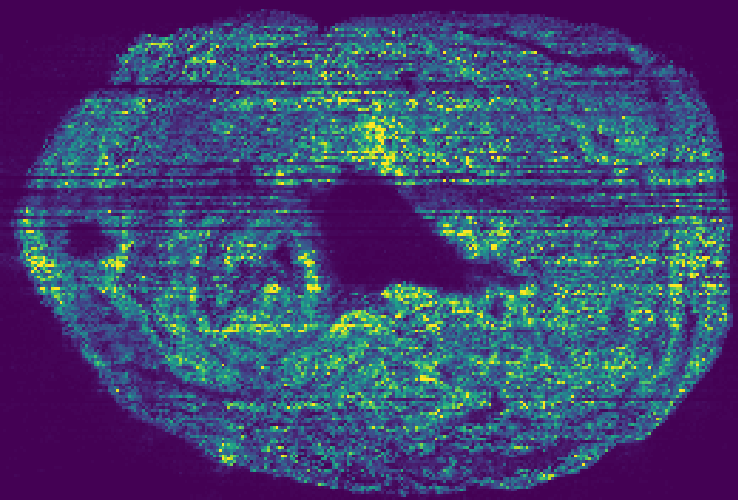
\includegraphics[width=\textwidth,height=4cm,keepaspectratio]{on_sample_1.png}
            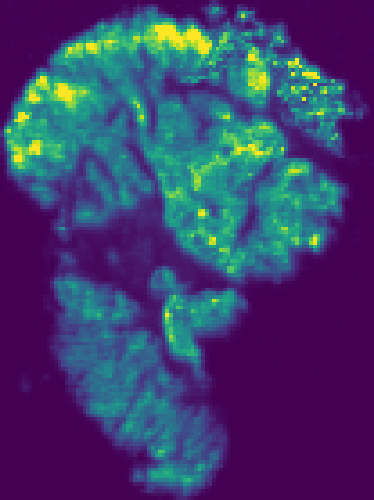
\includegraphics[width=\textwidth,height=4cm,keepaspectratio]{on_sample_2.png}
            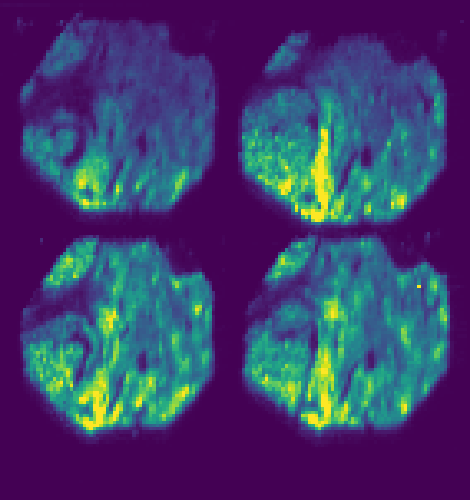
\includegraphics[width=\textwidth,height=4cm,keepaspectratio]{on_sample_3.png}
            \caption{On sample ion images}
        \end{subfigure}
        \begin{subfigure}[b]{\textwidth}
            \centering
            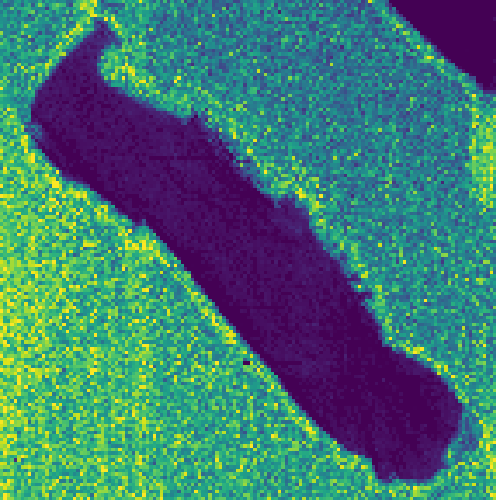
\includegraphics[width=\textwidth,height=4cm,keepaspectratio]{off_sample_1.png}
            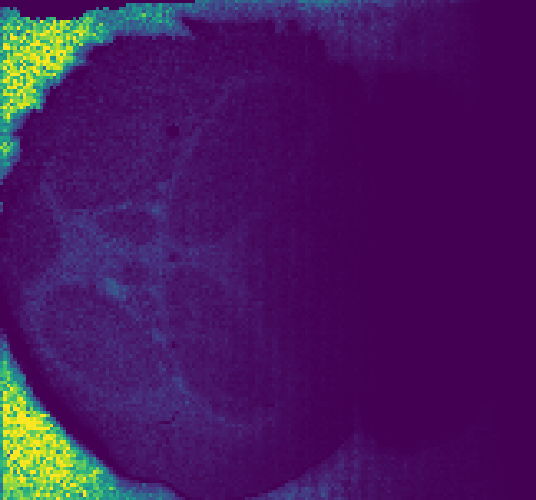
\includegraphics[width=\textwidth,height=4cm,keepaspectratio]{off_sample_2.png}
            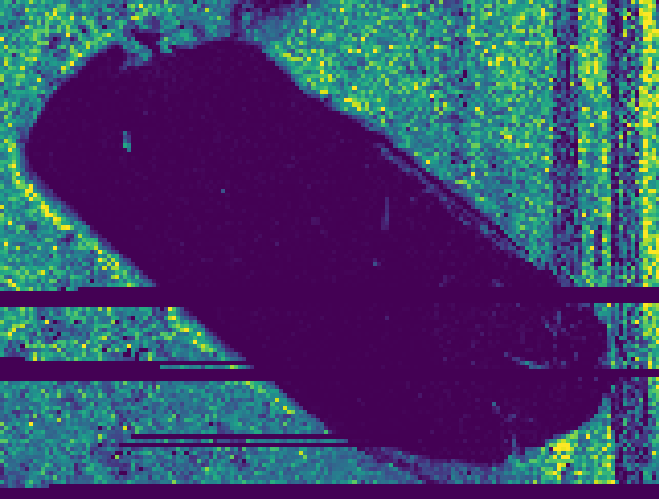
\includegraphics[width=\textwidth,height=4cm,keepaspectratio]{off_sample_3.png}
            \caption{Off sample ion images}
        \end{subfigure}
        \caption{Comparison of on sample (top) and off sample (bottom) ion images.}
    \end{figure}
    
    The final image distribution by classes:
    
    \begin{itemize}
        \item off sample - 7451
        \item on sample - 15665
    \end{itemize}
    
    \begin{figure}[H]
        \centering
            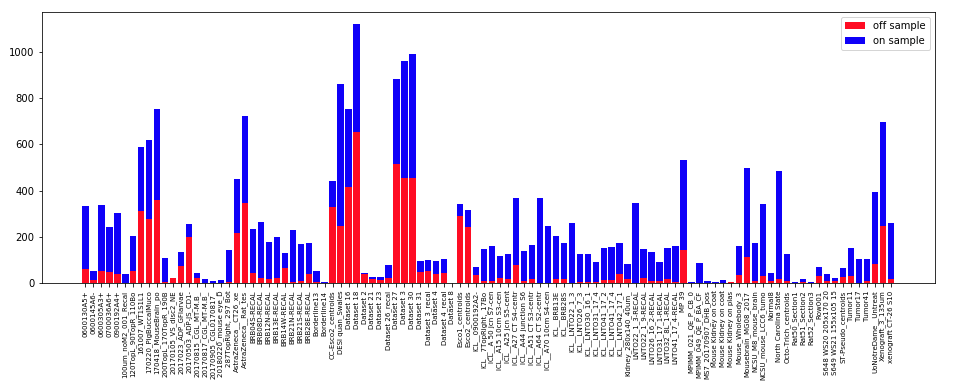
\includegraphics[width=\textwidth,height=7cm]{class_distribution.png}
        \caption{The final dataset appeared to be slightly unbalanced with approximately 30\%
        of target class images. But inside image groups (MSI datasets),
        image classes can be much more imbalanced.
        In some cases, a group has just a few images of the target class.
        This fact definitely added complexity to the problem.}
    \end{figure}
    
    As the next step, all the ion images were scaled into square images of $56 \times 56$ size.
    These images, grouped by MSI dataset they belong to, were used as inputs to the model.
    
    \subsection*{Implementation}
    
    A Convolutional Neural Network implemented in Keras with TensorFlow as a back-end was used as the model
    of choice for image classification. During model development the following questions have been explored:
    
    \begin{itemize}
        \item General CNN architecture decisions. How many convolutional and dense layers the model should have.
        As image features to be learned were not too complicated and number of classes was low, the network did
        not need to be too deep. Experiments confirmed that just four convolutional and three dense layers were enough.
        \item Number of units for each layers, the shapes of convolutional filters, size of strides and padding type
        were optimized with aim to have several hundreds thousand parameters to learn. At the same time, it was
        important to avoid excessive growth of parameters at the first dense layer.
        Large number of total network parameters also leads to network overfitting to easily.
        \footnote{Generalization: Peril of Overfitting 
            \url{https://developers.google.com/machine-learning/crash-course/generalization/peril-of-overfitting}}
        \item Types of activation functions. ReLU activation functions
        \footnote{Glorot, Xavier et al. "Deep Sparse Rectifier Neural Networks."
        AISTATS (2011)}
        proved to be effective and fast during backpropagation calculation. The problem of fading gradients
        affects them less than sigmoid or tahn functions.
        \item Number of max pooling layers was chosen to be half of convolutional layers number. Often in deep CNNs,
        only every second convolutional layer is followed by a max pooling layer. Here we followed the same rule.
        \item L2 regularization, use of dropout.
        \footnote{Srivastava, Nitish et al.
            "Dropout: A Simple Way to Prevent Neural Networks from Overfitting."
            Journal of Machine Learning Research 15 (2014).}
        L2 regularization did not help to improve the model accuracy but
        made it more stable while training. Use of dropout had some positive effects on model accuracy before
        batch normalisation was introduced after every convolutional layer. After that dropout was removed even
        from the dense layers.
        \item Batch normalisation
        \footnote{Szegedy, Christian et al.
            "Batch Normalization: Accelerating Deep Network Training by Reducing Internal Covariate Shift."
            arXiv preprint arXiv:1502.03167 ​(2015).}
        was added after every convolutional layer and greatly improved model accuracy
        and robustness. Normalising layer weights internally after every batch helps to improve model training
        speed as well. After adding it to the model it was enough to train the model for a couple of epochs.
        \item Loss function choice. Cross-entropy is recommended as an effective loss function for image classification
        tasks. In our case, we used binary cross-entropy as the task has two classes.
        \item Optimization algorithm and its hyperparameters. Experiments with a few different optimization algorithms
        has been done but the most effective appeared to be Stochastic Gradient Descent with momentum.
        Its hyperparameters were chosen during number of experiments and were close to those usually recommended
        ($learning\_rate=0.01$ and $momentum=0.9$).
        \item Model complexity evaluation and running time estimation. While optimizing the model architecture it was
        important to keep the number of parameters high but not increase their number too much as it is known to be prone 
        to overfitting. It was also important to keep running time under several minutes because otherwise
        it was not feasible to complete all experiments each of which included ten cross-validation runs
        with five repetitions for each cross-validation fold. More details below.
        \item Improving model robustness so that results do not change significantly between runs. From the very beginning, 
        due to some imbalance in the data mentioned above, the model results were slightly different after
        every training cycle on the same data. Lots of approaches have been explored in order to mitigate this issue.
        But eventually, the most effective one was just to train five different models on the same data and average their predictions.
    \end{itemize}
    
    \pagebreak
    The following steps represent complete process of building a model:
    
    \begin{enumerate}
        \item Select the number of convolutional and dense layers for the network.
        In our case, four layers was enough.
        \item Choose the activation function for all convolutional and dense layers.
        ReLU for all layers but the last one. Softmax for the last layer.
        \item Define the number of pooling layers. Every second convolutional layer
        is followed by a max pooling layer.
        \item Introduce batch normalisation into every convolutional layers.
        Batch normalisation is applied to the layer outputs before the activation function.
        \item Once the dimensions of resized images are defined, optimize the convolutional
        filter sizes, their number and strides so that the first dense layers does not get
        to many input values.
        \item Define the loss function. We recommend binary cross-entropy.
        \item Pick an optimization algorithm and optimize its parameters. Stochastic Gradient
        Descent with momentum proved to be the most effective for the problem.
        \item Select cross-validation scheme and use it to optimize all the hyperparameters
        of the network.
        \item Train the network with optimal hyperparameters on the all the data available and
        save it.
        \item Apply the saved network to the test data to measure the model performance on the
        test data.
    \end{enumerate}
    
    \begin{figure}[H]
        \centering
            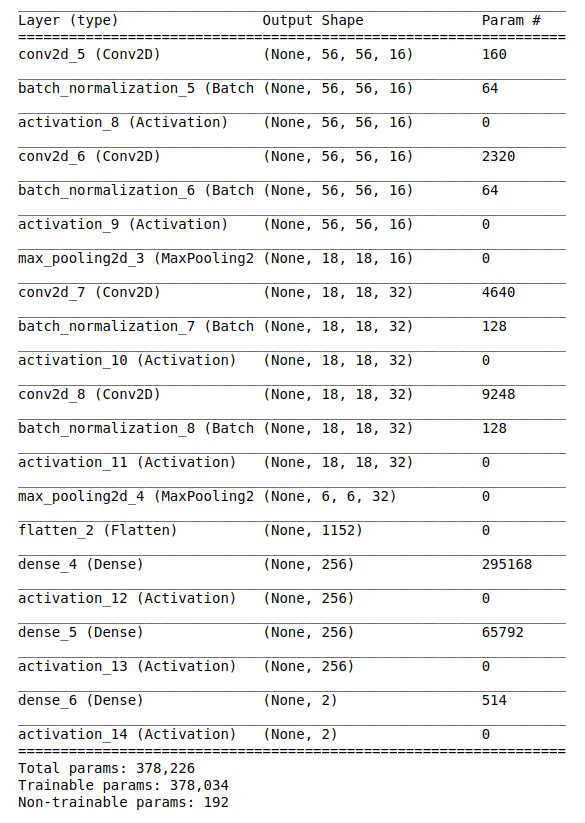
\includegraphics[width=\textwidth,height=16cm,keepaspectratio]{cnn_summary.png}
        \caption{The final network architecture}
    \end{figure}
    
    \pagebreak
    \section*{Results}
    
    \subsection*{Model Evaluation and Validation}
    
    The final model had four convolutional layers followed by three dense layers. All convolutional layers had batch
    normalisation applied. Every second one was followed by a max pooling layer. All activation functions were ReLU
    except for the last layer where softmax was used. Binary cross-entropy was used as the loss function. Stochastic
    Gradient Descent with momentum was used as the optimization algorithm.
    
    In order to evaluate robustness of the trained model, cross-validation technique was used. Because the dataset
    had internal groups of images, it was important to take this information into account when making cross-validation
    folds. Not following this approach resulted into model heavily overfitting due to information bleeding into the
    validation sets through similarities of the same group images presented in both train and validation sets.
    GroupKFold from scikit-learn Python package was used to implement correct cross-validation.
    
    Another challenge to be addressed was model robustness. The model kept providing slightly different results
    on the validation set being trained on the same train set. This fact made model accuracy evaluation and 
    hyperparameters optimization a more difficult task. All the attempts to add different types of regularization and 
    improve optimization algorithm did not help to alleviate completely this stochastic aspect of the model training.
    As a reasonable solution, it was decided to train the model five times on every train set (cross-validation fold)
    and save all five models in order to average their predictions on the validation and test sets.
    
    \begin{figure}[H]
        \centering
            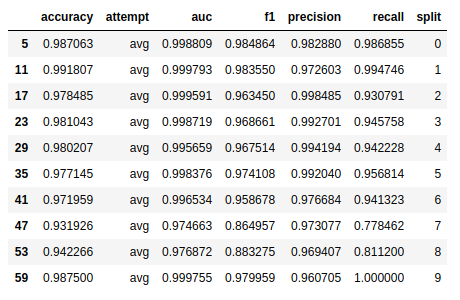
\includegraphics[width=\textwidth,height=6cm,keepaspectratio]{cross-validation_metrics.png}
        \caption{Group 10-fold cross-validation metrics}
    \end{figure}
    
    \begin{figure}[H]
        \centering
            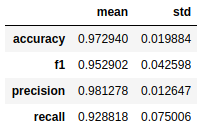
\includegraphics[width=\textwidth,height=2.5cm,keepaspectratio]{cross-validation_mean_metrics.png}
        \caption{Cross-validation mean metrics}
    \end{figure}
    
    \begin{figure}[H]
        \centering
            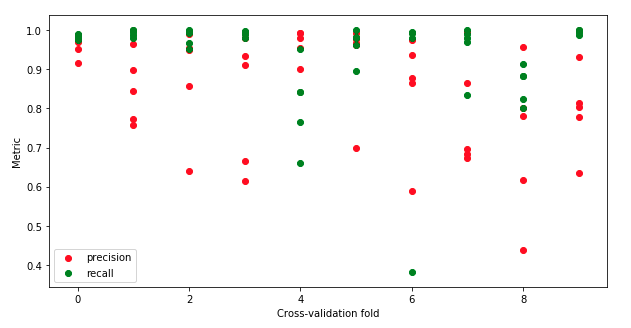
\includegraphics[width=\textwidth,height=10cm,keepaspectratio]{cross-validation_scatter_plot.png}
        \caption{Cross-validation metrics scatter plot}
    \end{figure}
    
    \subsection*{Justification}
    
    With use of Deep Convolutional Neural Networks it was possible to solve the problem in focus with higher accuracy
    ($recall=0.93\pm0.08, precision=0.98\pm0.01$) compared to the benchmark model ($recall=0.8, precision=0.75$).
    As for the original problem precision metric was more important, the final model provided substantially better solution.
    With achieved accuracy, the final model can be used in METASPACE project for filtering MSI dataset ion images
    that are not particularly interesting to the user.
    
    \pagebreak
    \section*{Conclusion}
    
    \subsection*{End Result Visualization}
    
    Examples of model predictions for a couple of completely new MSI datasets recently uploaded to METASPACE.
    
    \begin{figure}[H]
        \begin{subfigure}[b]{\textwidth}
            \centering
            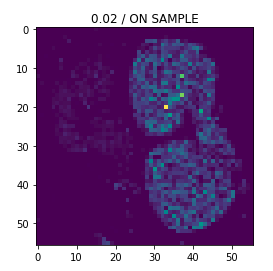
\includegraphics[width=\textwidth,height=5cm,keepaspectratio]{on_sample_test_pred_1.png}
            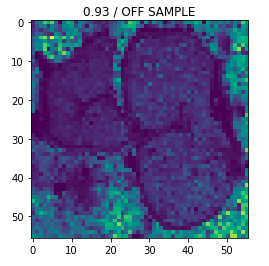
\includegraphics[width=\textwidth,height=5cm,keepaspectratio]{off_sample_test_pred_1.png}
            \caption{MSI dataset 1 predictions with target class probability and assigned label}
        \end{subfigure}
        \begin{subfigure}[b]{\textwidth}
            \centering
            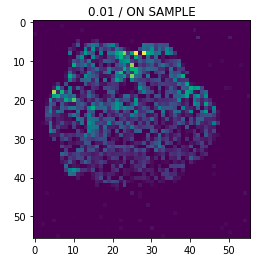
\includegraphics[width=\textwidth,height=5cm,keepaspectratio]{on_sample_test_pred_2.png}
            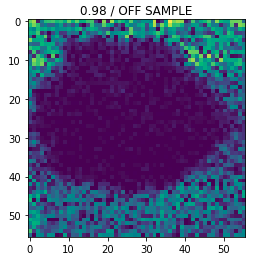
\includegraphics[width=\textwidth,height=5cm,keepaspectratio]{off_sample_test_pred_2.png}
            \caption{MSI dataset 2 predictions with target class probability and assigned label}
        \end{subfigure}
        \caption{Comparison of on sample ion images (left) with off sample ones (right).}
    \end{figure}
    
    \subsection*{Reflection}
    
    The process used for this project can be summarized the following way:
    
    \begin{enumerate}
        \item Initial problem formulation and setting the project goals.
        \item Data exploration and visualisation of separate MSI datasets.
        \item Attempts to use unsupervised learning, different versions of PCA and clustering algorithms,
        for separate MSI datasets in order to group their ion images into two classes.
        \item Using K-means clustering of MSI datasets spectra to learn off sample masks for all of them. Using this data as 
        ground truth data to train binary classification models to predict MSI dataset pixel class (on/off sample).
        Using this model as the benchmark model.
        \item Using expert knowledge to collect more than 23 thousands of labeled ion images from more than a hundred MSI datasets.
        \item Preprocessing of the ion images: image resizing, experimenting with data augmentation.
        \item Coming up with effective schema for the model validation.
        \item Optimizing the Convolutional Neural Network architecture and its hyperparameters.
        \item Training the final version of the model on all of the labeled data and applying it to some test data
        (absolutely new MSI dataset from METASPACE).
    \end{enumerate}
    
    The most surprising part of the project was to discover that predicting MSI dataset pixel classes with high accuracy
    is not enough for a good solution of the original problem where classification of ion images is needed.
    Having a dataset mask of off sample pixels is not enough, one should come up with a smart way 
    of combining this binary mask with each ion image in order to get a single number metric that
    would say how much the image looks like off sample area.
    Finding the right threshold for these metrics is also not an easy task as it heavily depends on a MSI dataset.
    
    The most useful part of the project was to try to solve a real world problem from the ground up.
    From defining the problem itself to coming up with a way to collect input data and labels,
    to large number of long running experiments with aim to find a network architecture that would work the best.
    As expected, it was quite difficult to find the right model and its parameter optimal values.
    But it was surprisingly easy to get from model that kind of works to a completely useless one.
    So the process of network optimization was definitely the toughest part of the project.
    
    \subsection*{Improvement}
    
    Probably the first issue to be addressed for the described solution is the model robustness.
    The fact that model fits its parameters quite differently on the same train set every time
    training is done simply does not appeal, especially when one considers moving this solution
    into a production system. A potential solution can be in finding a better
    way of initializing network parameters or choosing a better optimizer.
    Perhaps, exploring other deep learning frameworks
    can provide other options that are not available in TensorFlow.
    
    One of the issues of the CNN based solution is sensitivity.
    Model accuracy heavily depends on test MSI dataset.
    On some of them the result is close to 100\%, on others it can be as bad as 50-60\%.
    Using an ensemble of models, with CNN as one of them,
    will help to exploit different information hidden in the available data.
    Combining predictions of several independent models might improve the accuracy and 
    robustness of the final solution.
    
    \end{document}